\section{Recorded Resource Study and Precision Sensitivity}\label{sec:resources}
\subsection{Compact simulation and native circuits solve different accounting tasks}
The compact selector represents only fixed-cardinality subsets. Its complex128 amplitude array uses $16F$ bytes, where $F=\binom{15}{8}$ for the base or $F=\binom{M}{3}$ for refinement. This allocation excludes stored coefficients, energies, candidate features, and process memory. A full $\nu$-qubit statevector would instead require $16\,2^\nu$ bytes for amplitudes alone. Neither expression measures total system memory.

Compact simulation enumerates basis energies before amplification, so its objective evaluations must be counted separately from incumbent checks, measured trials, and logical phase calls. The recorded convention assigns two reversible objective calls to a phase operation for compute and uncompute. Constraint evaluation, state preparation, reflection, and physical data access would add work to an actual circuit execution. A logical query count does not capture all of these costs.

The native study uses 32 saved training queries per collection, drawn from the confirmation samples. It evaluates five compact-search seeds, tail pools of 3, 5, 8, 12, 16, or 20 candidates, and pair precisions of 4, 8, 12, or 16 bits. Its 178 completed tasks include 80 native synthesis cells. Actual pool availability is retained: a requested size unavailable for a real query is not silently replaced by a smaller pool. Artificial stress instances at the specified larger sizes are labeled separately.

The study was completed before this journal manuscript. It provides neither new relevance judgments nor another full-test evaluation. Its controlled subpools retain the original tail, and native representatives are the first two eligible frozen seed-zero queries for a dataset/pool, when available. The representatives remain fixed across precisions. Comparisons across pool sizes may nevertheless involve different eligible queries, so growth curves describe the measured cells rather than a random population scaling law.

\subsection{Reversible constraint and objective registers}
Writing $x_i\in\{0,1\}$ for a remaining tail candidate, the integer refinement objective has the polynomial form
\begin{equation}
E(x)=C_H+\sum_i\alpha_i x_i+\sum_{i<j}\alpha_{ij}x_ix_j,
\label{eq:native_polynomial}
\end{equation}
where $C_H$ contains fixed head--head terms, $\alpha_i$ sums rounded head--candidate terms, and $\alpha_{ij}$ represents a rounded candidate pair. The oracle evaluates signed improvement relative to the incumbent and marks only states with cardinality three and all three threshold-count conditions in~\eqref{eq:threshold_counts}.

The register allocation comprises $M$ decision qubits, $w$ signed-value qubits, $c=\lceil\log_2(M+1)\rceil$ counter qubits, $c-1$ comparator workspace qubits, and four constraint flags. Thus,
\begin{equation}
\nu=M+w+2c+3.
\label{eq:logical_width}
\end{equation}
The signed width must bound the objective difference on all bit strings, including states with invalid cardinality. Designing $w$ from valid three-element subsets alone could permit overflow on states the circuit must process before rejecting them. The implementation bounds the full polynomial domain and includes every workspace register in the reported total.

The oracle computes objective and constraints, conditionally applies the phase, and reverses the computation. The same counter and comparison workspace can be reused for successive threshold checks, while their flags are retained until phase marking. This structure explains both the logical-width formula and why a compact classical basis dimension is not an interchangeable qubit count.

\begin{table}[t]
\centering\small\setlength{\tabcolsep}{3pt}
\caption{Recorded native-oracle synthesis summary. Slash-separated entries compare 4/16-bit coefficients; full four-precision measurements are retained in the accompanying native CSV. Width includes workspace. Depth and CX values are maxima over the stated bounded sample; stress rows are artificial.}
\label{tab:native}\begin{tabular}{rlrrr}
\toprule
Tail & Source & Qubits & Depth & CX gates\\
\midrule
3 & real & 19/31 & 1049/1865 & 992/2408\\
5 & real & 23/35 & 3891/5955 & 3256/6160\\
8 & real & 29/41 & 15067/20722 & 11684/18240\\
12 & real & 34/46 & 27570/41294 & 22068/36076\\
16 & stress & 39/51 & 61665/67687 & 43628/52212\\
20 & stress & 43/55 & 79769/96137 & 58220/75556\\
\bottomrule
\end{tabular}

\end{table}

Table~\ref{tab:native} summarizes the measured cells. Figure~\ref{fig:native} includes all four precision levels and distinguishes real samples from artificial stress cases. Synthesis uses the unrestricted $u,\mathrm{cx}$ basis, optimization level one, and transpiler seed zero. These are logical resources without coupling-map routing, device calibration, or error correction. The gate count therefore cannot be described as the cost of execution on a particular processor.

\begin{figure*}[t]
\centering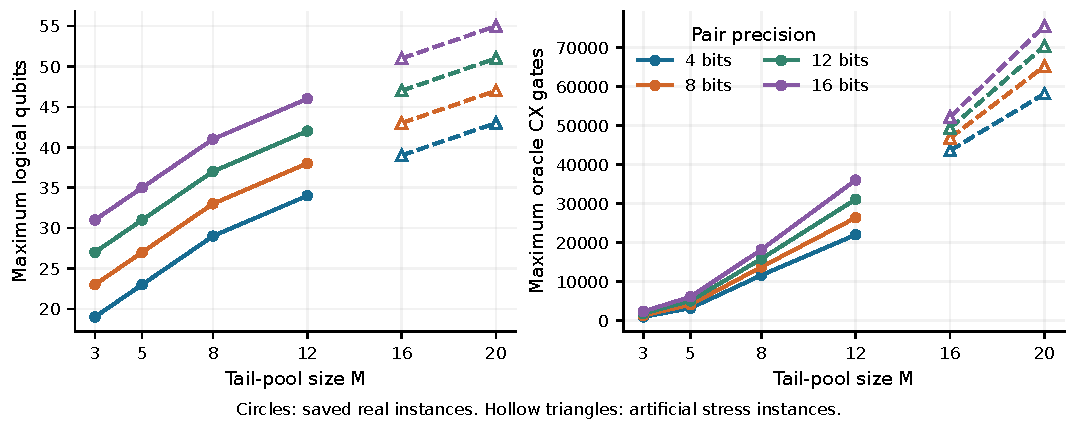
\includegraphics[width=\textwidth]{native_resources.pdf}
\caption{All recorded precision levels for native logical width and oracle CX count. Real-instance points summarize the available fixed representatives; hollow triangles are artificial stress cells. Connecting lines aid inspection and are not fitted scaling models.}
\label{fig:native}
\end{figure*}

\subsection{Precision and search error}
The coefficient bound in~\eqref{eq:refinement_bound} decreases with $b$. The observed GAS output can nevertheless have a larger gap to the exact float optimum because a finite search budget need not find the exact integer optimum. Figure~\ref{fig:precision} separates this empirical search outcome from a statement about coefficient approximation. The saved float gap is the output redundancy minus the exact admissible float optimum for that instance; the quantized gap uses the exact encoded optimum.

\begin{figure*}[t]
\centering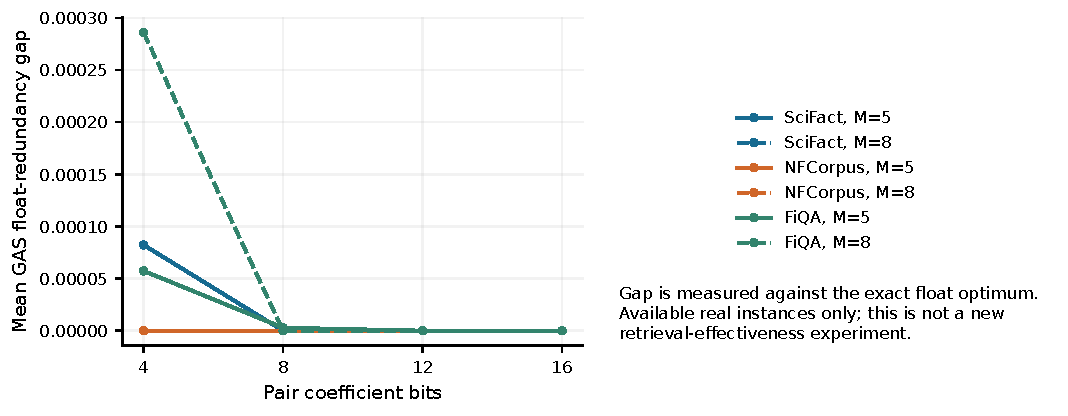
\includegraphics[width=\textwidth]{precision_gaps.pdf}
\caption{Recorded GAS float-redundancy gaps across pair precision for available real five- and eight-candidate subpools. Values are means over the study's fixed available requests, not new retrieval runs. Search error can dominate coefficient error; the exact-optimizer regret bound does not bound these GAS curves.}
\label{fig:precision}
\end{figure*}

Greater precision may distinguish more objective values while increasing signed arithmetic width and circuit work. It does not necessarily yield a monotone improvement in a stochastic, budget-limited output. Nor does a smaller optimization gap imply improved judged relevance: the objective still penalizes pair similarity subject to estimated-score constraints. This is why the primary paper reports retrieval metrics, exact objective controls, and resources together.

\subsection{Validation coverage and explicit limits}
Complete-iteration synthesis, including generic fixed-weight preparation and reflection, is limited to at most eight decision qubits. Native validation simulation is limited to at most five decisions. Six complete iterations passed phase-sensitive validation; 42 other simulation attempts were refused by the conservative memory guard. These refusals mark the limits of the simulations; they do not demonstrate successful execution of larger circuits. Separate small two-bit toy checks exercise nontrivial five-decision marking and reflection.

The native simulator uses a noiseless matrix-product-state method with zero configurable truncation threshold, maximum bond dimension 128, and a $10^{-8}$ probability tolerance. An independently constructed expected-state inverse followed by local $Z$ expectations bounds state mismatch and workspace leakage. Every circuit worker has 120-second and 2\,GiB limits. Larger native simulations, a noise sweep, hardware routing, and physical execution remain unperformed.

Construction, transpilation, native validation, compact selection, allocation profiling, and complete-pipeline timing have different boundaries. Per-method allocation profiling is a separate replay excluded from selector timing, while the fresh worker's process RSS covers its complete grid. Keeping these boundaries separate prevents an allocation replay from inflating one reported time while a costly prerequisite disappears from another.
